% Project:  TeX Cover Letter Template
% Author:   Sid Lacy

% EDIT info.tex, body.tex

\documentclass{article}
\usepackage[utf8]{inputenc}
\usepackage[empty]{fullpage}
\usepackage[hidelinks]{hyperref}
\usepackage{graphicx}
\usepackage{fontawesome5}
\usepackage{eso-pic}
\usepackage{charter}
\usepackage{subcaption}
\usepackage{float}
\addtolength{\topmargin}{-0.5in}
\addtolength{\textheight}{1.0in}
\definecolor{gr}{RGB}{225,225,225}
\usepackage{longtable}  % Cargar el paquete longtable





%% end info---------------------------------------------------------------

\begin{document}

\setlength\parindent{24pt}







\small

     \includegraphics[width=0.3\textwidth]{/home/pgaisse/asesoreseprime/src/public/style-1/img/logo_p.png}
                        \begin{center}
                        \textbf{\underline{\LARGE Informe de Reparaciones}}
                        \end{center}

                        \textbf{\underline{Datos del Asegurado}}
                        \begin{itemize}
                        \item Nombre:  Erick Alfonso Soza Palma
                        \item Rut: 17.039.281-7
                        \item Dirección: 43 Oriente B  268, Hacienda Las Rastras
                        \item Ciudad: Talca
                        \item Email: ericksoza@gmail.com
                        \item Fono: 989952139
                        \end{itemize}
                        
                        \textbf{\underline{Antecedentes del Siniestro}}\par
                        \begin{itemize}
                        \item Tipo de Siniestro: Rotura de ca?erias
                        \item Siniestro: Rotura de ca?erias
                        \item Fecha del Siniestro: 2022-02-05
                        \item Intensidad: M
                        \item Información adicional: Inundaciones en la ciudad X debido a lluvias intensas
                        \end{itemize}\begin{center}\large\textbf{Fachada}\end{center}
                        \begin{figure}[H]
                        \centering
                        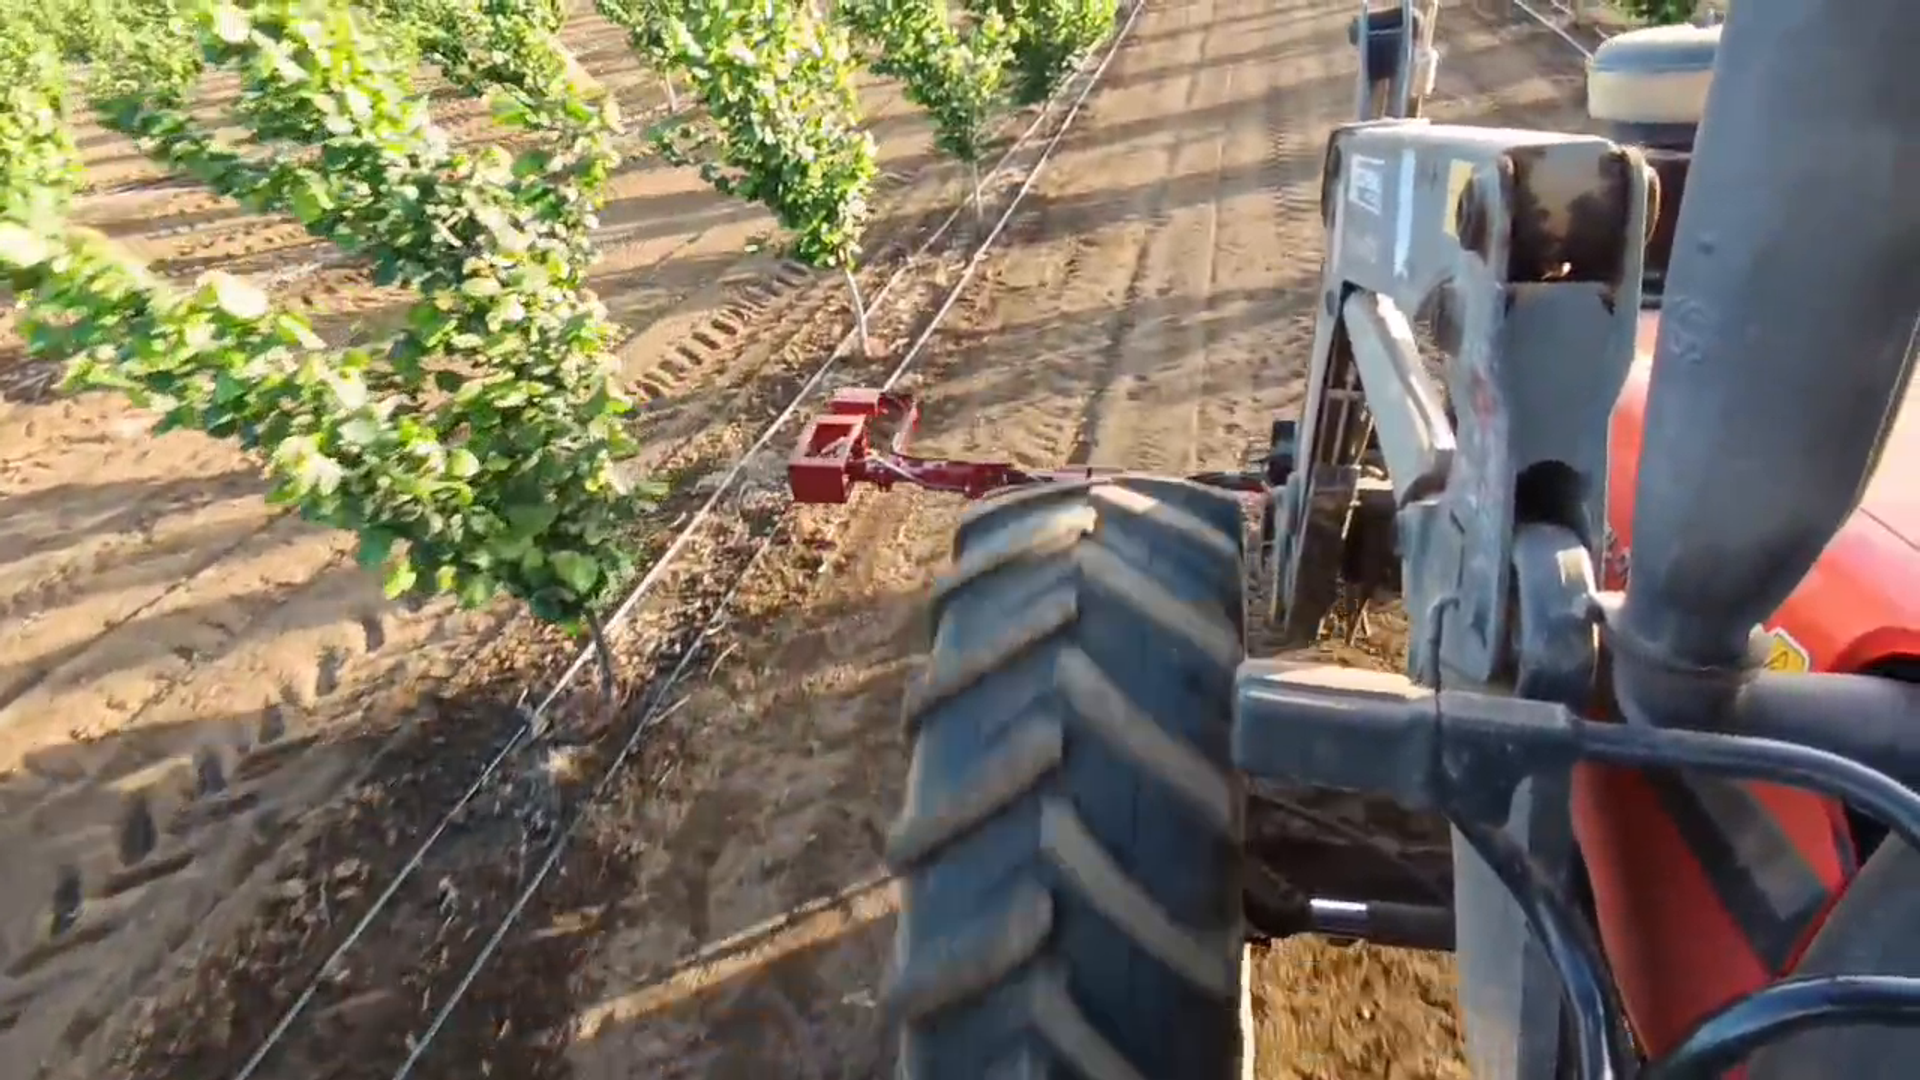
\includegraphics[width=200 px,height=112.5 px]{/home/pgaisse/asesoreseprime/src/public/uploads/images/img_m/26c0eaba-a86a-4958-b1a5-0a5e4c07e2b3.png}
                        \hspace{0.5cm}
                        \includegraphics[width=200 px,height=112.5 px]{/home/pgaisse/asesoreseprime/src/public/uploads/images/img_m/a5fa4577-1419-4867-a18a-5b93210f37da.png}
                        \end{figure}\begin{center}\large\textbf{Pasillo} (Ancho: 45, Largo: 30, Alto : 323).\end{center}\par
      \par 
                    \begin{figure}[H]
                    \centering
                    \includegraphics[width=200 px,height=112.5 px]{/home/pgaisse/asesoreseprime/src/public/uploads/images/img_m/ef1a567c-d351-4037-8850-307974e454e3.png}
                    \hspace{0.5cm}
                    \includegraphics[width=200 px,height=112.5 px]{/home/pgaisse/asesoreseprime/src/public/uploads/images/img_m/afde993c-cc45-4deb-9efe-de6eb9aa2e95.png}
                    \end{figure} \begin{center}\textbf{{\large Daños presentados en Pasillo}}\end{center} \textbf{\underline{Picoteo de gallina}} (Cantidad de daño : 20 uni).\par
      \par\vspace{0.5cm}
                \begin{figure}[H]
                \begin{subfigure}[b]{0.3\textwidth}\centering\includegraphics[width=120 px,height=67.5 px]{/home/pgaisse/asesoreseprime/src/public/uploads/images/img_m/4d865c7e-95b0-4973-a3c3-7cc407c3bc22.png}\end{subfigure}
                \begin{subfigure}[b]{0.3\textwidth}\centering\includegraphics[width=120 px,height=67.5 px]{/home/pgaisse/asesoreseprime/src/public/uploads/images/img_m/8bbdcffe-8ef9-4fd0-a737-050fad37095a.png}\end{subfigure}
                \begin{subfigure}[b]{0.3\textwidth}\centering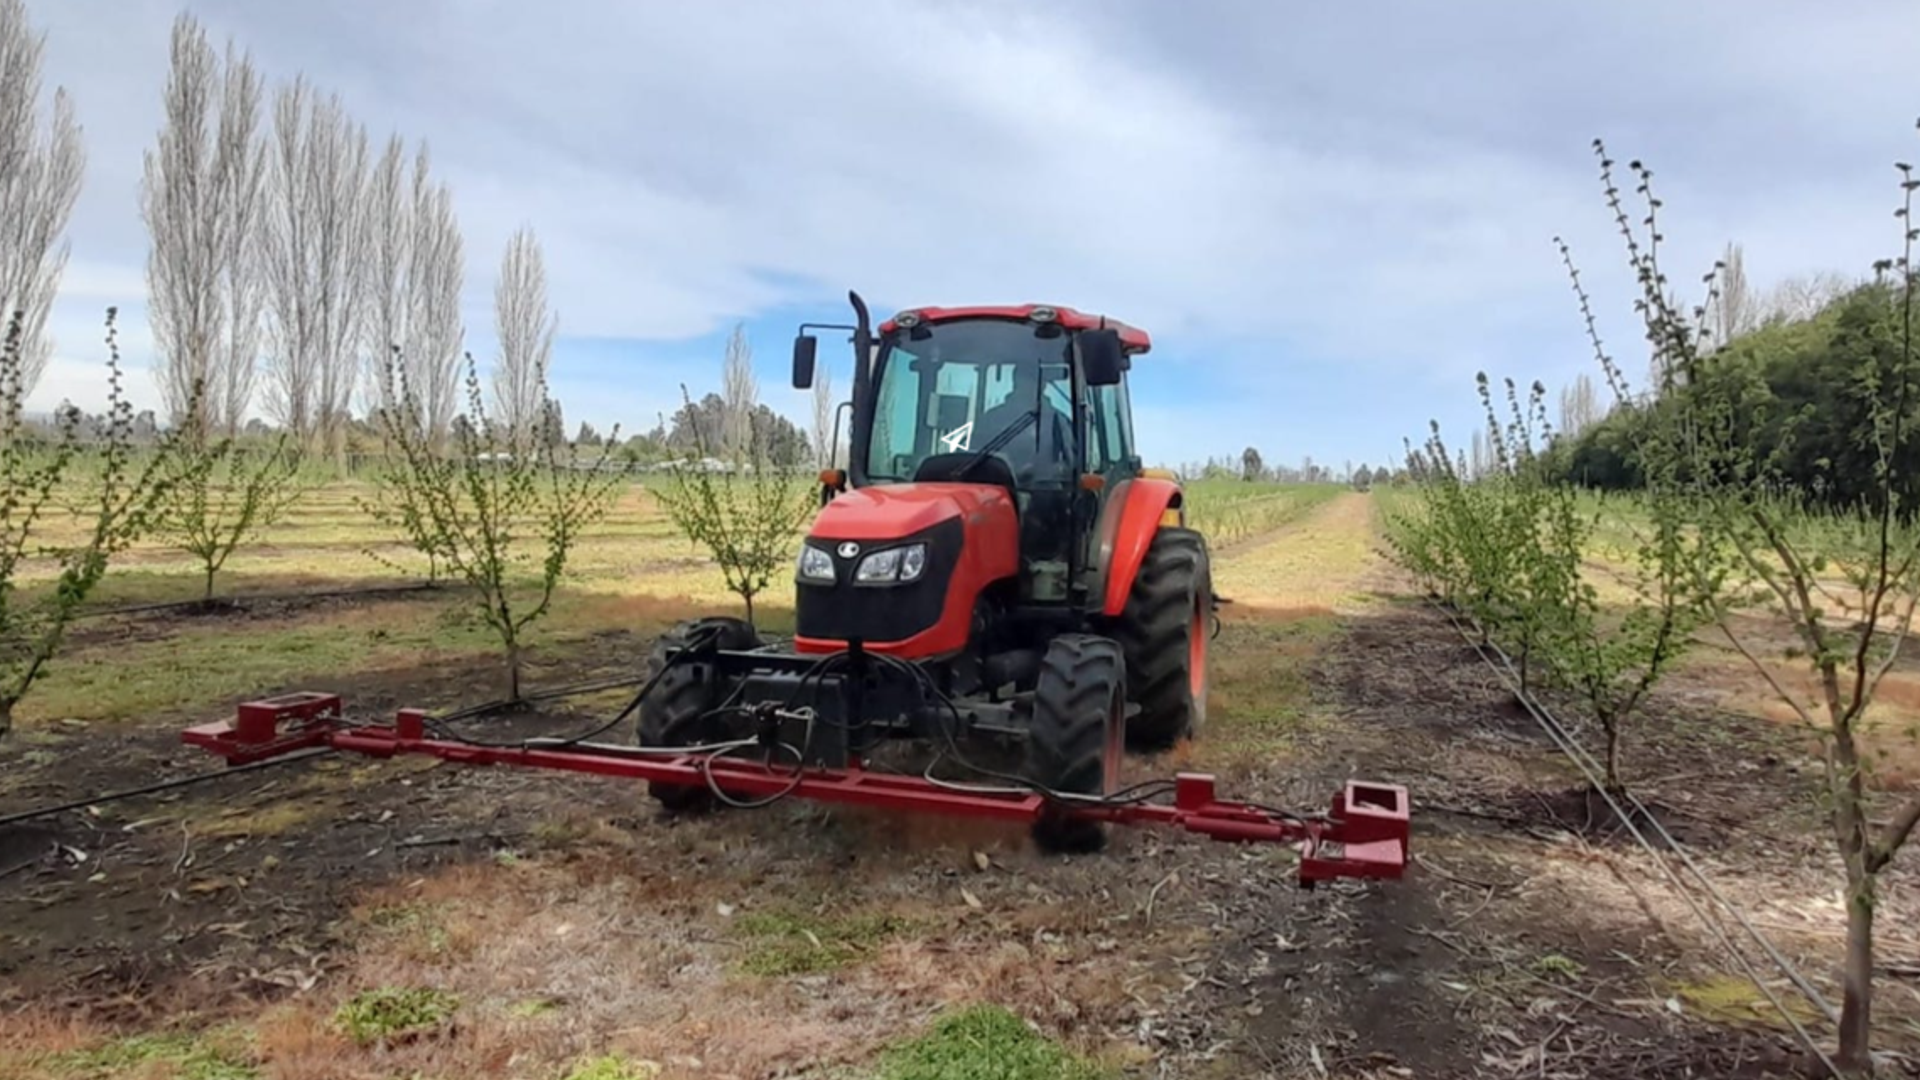
\includegraphics[width=120 px,height=67.5 px]{/home/pgaisse/asesoreseprime/src/public/uploads/images/img_m/68dea519-4ed5-4c61-8021-1cc5d90ddb27.png}\end{subfigure}
            \end{figure}\begin{center}\large\textbf{Pasillo} (Ancho: 45, Largo: 30, Alto : 323).\end{center}\par
      \par 
                    \begin{figure}[H]
                    \centering
                    \includegraphics[width=200 px,height=112.5 px]{/home/pgaisse/asesoreseprime/src/public/uploads/images/img_m/bf105b31-e9c4-434e-8de7-3f4ecdd2faa3.png}
                    \hspace{0.5cm}
                    \includegraphics[width=200 px,height=112.5 px]{/home/pgaisse/asesoreseprime/src/public/uploads/images/img_m/eb23dea6-7701-458b-a1e9-6ff67f335577.png}
                    \end{figure} \begin{center}\textbf{{\large Daños presentados en Hall de acceso}}\end{center} \textbf{\underline{Fisura en muro}} (Cantidad de daño : 20 mm).\par
      \par\vspace{0.5cm}
                \begin{figure}[H]
                \begin{subfigure}[b]{0.3\textwidth}\centering\includegraphics[width=120 px,height=67.5 px]{/home/pgaisse/asesoreseprime/src/public/uploads/images/img_m/d306dfb9-c4b9-4aae-9204-3b236d193370.png}\end{subfigure}
                \begin{subfigure}[b]{0.3\textwidth}\centering\includegraphics[width=120 px,height=67.5 px]{/home/pgaisse/asesoreseprime/src/public/uploads/images/img_m/5c74867b-f4aa-4c9c-892b-4d2c8bbdeb14.png}\end{subfigure}
                \begin{subfigure}[b]{0.3\textwidth}\centering\includegraphics[width=120 px,height=67.5 px]{/home/pgaisse/asesoreseprime/src/public/uploads/images/img_m/634c2c70-168c-47bf-ada3-904a5bdee050.png}\end{subfigure}
            \end{figure}


% Closer
\vspace{0.1in}
\vfill

\begin{flushright}

\vspace{-0.1in}\includegraphics[width=1.5in, draft=false]{/home/pgaisse/asesoreseprime/src/public/uploads/images/img_m/2ce8b5dd-eb5e-4dea-914f-23a7e0e36eba.png}\vspace{-0.1in}

\end{flushright}

\end{document}